\documentclass[a4paper, 12pt]{article}
\usepackage[english, russian]{babel}
\usepackage{svg}
\usepackage[T2A]{fontenc}
\usepackage[utf8]{inputenc}
\usepackage{ stmaryrd }
\usepackage{ dsfont, amsmath, amsfonts, amssymb, amsthm, mathtools }
\theoremstyle{plain}
\newtheorem{theorem}{Теорема}
\newtheorem{lemma}{Лемма}
\newtheorem{definition}{Определение}
\usepackage[english, russian]{babel}
\usepackage[T2A]{fontenc}
\usepackage[utf8]{inputenc}
\usepackage{amssymb}
\usepackage{amsfonts}
\usepackage{geometry}
\geometry{top=15mm}
\geometry{bottom=15mm}
\geometry{left=15mm}
\geometry{right=15mm}
\linespread{1.3}
\usepackage{graphicx}
\usepackage{graphicx}
\usepackage{setspace}
\usepackage{amsmath}
\usepackage{tikz}
\usetikzlibrary{graphs}
\usepackage{amscd}
\usepackage[all]{xy}

\begin{document}
	\setcounter{page}{1}
	
	\begin{center} 
		\textbf{Правительство Российской Федерации}
		\\ \textbf{Федеральное государственное автономное образовательное учреждение}
		\\ \textbf{высшего профессионального образования}
		\\ \textbf{«Национальный исследовательский университет»}
		\\ \textbf{«Высшая школа экономики»}
		\\ \textbf{Нижегородский кампус}
		\vspace{3cm}
		\\ Факультет математики, информатики и компьютерных наук
		\\ Кафедра фундаментальной математики
		\vspace{3cm}
		\\ \large\textbf{КУРСОВАЯ РАБОТА}
		\vspace{0.3cm}
		\\ \large\textbf{ВИЗУАЛИЗАЦИЯ ГРАДИЕНТНО-ПОДОБНОГО КАСКАДА НА СФЕРЕ ПО ЕЁ ТРЁХЦВЕТНОМУ ГРАФУ}
	\end{center}
	
	\vspace{3cm}\hspace{8cm} Выполнил: 
	\par \hspace{8cm} Студент 2 курса группы 22 ФМ 
	\par \hspace{8cm} Турсунов Данил Вячеславович
	\par \vspace{0.8cm} \hspace{8cm} Научный руководитель:
	\par \hspace{8cm} Баринова Марина Константиновна
	\begin{center} 
		\vspace{4cm} Нижний Новгород
		\par Май 2024 г.
	\end{center}
	
	\newpage
	\begin{center}
		\LARGE\textbf{Содержание}
	\end{center}
	\newpage

	\textsf{Hello everyone!}
	\section{Вступление}
	\subsection{Цели и задачи работы}
		Основной целью работы является создание приложения на языках C++ и Python с применением библиотеки Manim. Суть приложения заключается в генерации 3D-изображений градиентно-подобных каскадов, заданных на сфере, из соответствующих им трёхцветных графов, заранее проверенных программой на корректность. Алгоритмическая часть приложения написана на C++, так как этот язык в разы быстрее чем язык Python, а на языке Python написана визуальная составляющая программы, так как язык содержит множество удобных для этого библиотек. Помимо этого поставлены следующие подзадачи: $\\$
		1) Разобраться в связи градиентно-подобных каскадов и трёхцветных графов;$\\$
		2) Научиться писать Unit-тесты на языке C++, необходимые для стабильной работы программы при её изменении в дальнейшем;$\\$
		3) Придумать алгоритм генерации трёхцветных графов с заданными параметрами: число Эйлера и число сёдел динамической системы.
	\subsection{Актуальность работы}
		Программа, написанная в результате работы, будет полезна начинающим научным сотрудникам или обычным студентам, желающим разобраться в градиентно-подобных каскадах на сфере, так как она поможет им быстрее визуализировать эти динамические системы. Помимо этого, отдельные функции из алгоритмический части могут быть полезны другим исследователям трёхцветных графов в написании программ.
	\section{Теоретическая часть}
	\subsection{Описание}
	В этой главе будет представлено построение трёхцветного графа по градиентно-подобному каскаду на поверхности. Стоит отметить, что на языке трёхцветных графов получена полная топологическая классификация градиентно-подобных каскадов на поверхностях.
	\subsection{Трёхцветный граф как полный топологический инвариант диффеоморфизма на поверхности}
	\begin{definition}
		Диффеоморфизм $f: M^n \shortrightarrow M^n$, заданный на гладком замкнутом n-многообразии, называется диффеоморфизмом Морса-Смейла, если:$\\$
		1) неблуждающее множество $\Omega_f$ гиперболично и конечно (т.е. состоит из конечного чила периодических точек, для которых модули собственных значений матрицы Якоби не равны единице);$\\$
		2) для любых периодических точек p, q устойчивое многообразие $W^s_p$ и неустойчивое многообразие $W^u_q$ либо не пересекаются, либо трансверсальны в каждой точке пересечения.
	\end{definition}
	Пусть $f: M^n \shortrightarrow M^n$ - диффеоморфизм Морса-Смейла, тогда периодические точки называются источниками, если неустойчивое многообразие $W^u_q$ имеет размерность $n$, стоками, если $0$, и сёдлами при остальных. $\\$
	Далее скажем, что для любой периодической точки $p$ диффеоморфизма $f$ компоненты связности $W^s_p \textbackslash p~(W^u_p \textbackslash p)$ называются её устойчивыми (неустойчивыми) сепаратрисами. $\\$
	Рассмотрим класс диффеоморфизмов на поверхности $M^2$, тогда диффеоморфизм Морса-Смейла называется градиентно-подобным, если $W^s_p \cap W^u_p = \o$ для любых различных седловых точек $p,q$. $\\$
	В дальнейшем в работе будут рассматриваться исключительно граентно-подобные диффеоморфизмы, заданные на поверхности $M^2$. $\\$
	Удалим из поверхности $M^2$ замыкание объединения устойчивых и неустойчивых многообразий седловых точек $f$ и получим множество $M' = M^2 \textbackslash (W^{u}_{\Omega^0_f} \cup W^{u}_{\Omega^1_f} \cup W^{s}_{\Omega^1_f} \cup W^{s}_{\Omega^2_f})$. $\\$
	$M'$ является объединением ячеек, гомеоморфных открытому двумерному диску, граница которых имеет один из 3-х следующих видов: (КАРТИНКА С ЯЧЕЙКАМИ) $\\$
	Пусть $A$ - ячейка из $M'$, $\alpha$ и $\omega$ - источник и сток, входящие в её границу. Кривую $\tau\in A$, началом и концом которой являеются $\alpha$ и $\omega$, будем называть $t-$кривой. Через $T$ обозначим множество $t-$кривых, взятых по одной из каждой ячейки. $\\$
	Разобьём каждую ячейку этой кривой на 2 области, компоненты связности $M_\Delta = M' \textbackslash T$ назовём треугольными областями. Через $\Delta_f$ обозначим множество всех областей диффеоморфизма $f$. В границу каждой треугольной области входят 3 периодические точки: источник, сток и седло, а также устойчивая сепаратриса, неусточивая сепаратриса и кривая $\tau$. В дальнейшем будем называть их $s-$кривой, $u-$кривой и $t-$кривой соответственно. Замыкание каждой из этих кривых будем называть стороной треугольной области. Скажем, что сторона является общей стороной для двух треугольных областей, если она принадлежит замыканиям этих треугольных областей. $\\$
	Для дальнейшего введения в теорию, потребуется ввести несколько определений из теории графов.
	\begin{definition}
		Конечным графом называется упорядоченная пара (B,E), для которой выполнены следующие условия: $\\$
		1) B - непустое конечное множество вершин; $\\$
		2) E - множество пар вершин, называемых рёбрами.
	\end{definition}
	\begin{definition}
		Если граф содержит ребро e = (a,b), то каждую из вершин a, b называют инцидентной ребру e и говорят, что вершины a и b соединены ребром e.
	\end{definition}
	\begin{definition}
		Путём в графе называют конечную последовательность его вершин и рёбер вида: $b_0, (b_0, b_1), b_1, \dots, b_{i-1}, (b_{i-1}, b_{i}), b_{i}, \dots, b_{k-1}, (b_{k-1}, b_{k}), b_{k}, k >= 1$. Число k называется длиной пути, оно совпадает с числом входящих в него рёбер.
	\end{definition}
	\begin{definition}
		Граф называют связным, если любые две его вершины можно соединить путём.
	\end{definition}
	\begin{definition}
		Циклом длины $k \in \mathds{N}$ в графе называют конечное подмножество его вершин и рёбер вида \{$b_0, (b_0, b_1), b_1, \dots, b_{i-1}, (b_{i-1}, b_{i}), b_{i}, \dots, b_{k-1}, (b_{k-1}, b_{0})$\}. Простым циклом называют цикл, у которого все вершины и рёбра попарно различны.
	\end{definition}
	С учётом имеющихся у нас вводных, введём определение трёхцветного графа, а также сформулируем некоторые теоремы.
	\begin{definition}
		Граф T называется трёхцветным графом, если: $\\$
		1) множество рёбер графа T является объединением трёх подмножеств, каждое из которых состоит из трёх рёбер одного и того же определенного цвета (цвета рёбер из разных подмножеств не совпадают, будем обозначать эти цвета буквами s, t, u, а рёбра для краткости будем называть s-, t-, u-рёбрами); $\\$
		2) каждая вершина графа T инцидентна в точности трём рёбрам различных цветов;$\\$
		3) граф не содержит циклов длины 1.
	\end{definition}
	\begin{definition}
		Простой цикл трёхцветного графа T назовём двухцветным su-, tu- или st-циклом, если он содержит рёбра в точности двух цветов s и u, t и u, s и t соответственно.
	\end{definition}
	 Непосредственно из определения трёхцветного графа следует, что длина любого двухцветного цикла является чётным числом (так как цвета рёбер строго чередуются), а отношение на множестве вершин, состоящее в принадлежности двухцветному циклу определённого типа, является отношением эквивалентности, то есть каждая отдельно взятая вершина лежит в точности в одном  $su-$, одном $tu-$ и одном $st-$цикле.
	\begin{definition}
		Построим трёхцветный граф $T_f$, соответствующий диффеоморфизму $f \in G$, следующим образом:$\\$
		1) вершины графа $T_f$ взаимно однозначно соответствуют треугольным областям множества $\Delta$; $\\$
		2) две вершины графа инцидентны ребру цвета s, t, u, если соответствующие этим вершинам треугольные области имеют общую s-, t- или u-кривую .
	\end{definition}
	Граф $T_f$ полностью удовлетворяет определению трёхцветного графа.
	\begin{theorem}
		Теорема 1. Для того чтобы диффеоморфизмы f, f' из класса G были топологически сопряжены, необходимо и достаточно, чтобы их графы ($T_f, P_f$) и ($T_{f'}, P_{f'}$) были изоморфны.
	\end{theorem}
	\begin{definition}
		Определение 2. Трёхцветный граф (T,P) назовём допустимым, если он обладает следующими свойствами: $\\$
		1) граф T связен;$\\$
		2) длина любого su-цикла графа T равна 4; $\\$
		3) автоморфизм P является периодическим.
	\end{definition}
	\begin{lemma}
		Пусть $f \in G$. Тогда трёхцветный граф ($T_f, P_f$) является допустимым.
	\end{lemma}
	\begin{theorem}
		Пусть (T,P) - допустимый трёхцветный граф. Тогда существует диффеоморфизм $f:M^2 \shortrightarrow M^2$ из класса G, граф ($T_f, P_f$) которого изоморфен графу (T,P). При этом: $\\$
		1) эйлерова характеристика поверхности $M^2$ вычисляется по формуле $X(M^2) = v_0 - v_1 + v_2$, где $v_0, v_1, v_2$ - число всех tu-, su-, st-циклов графа T соответственно; $\\$
		2) поверхность $M^2$ ориентируема тогда и только тогда, когда все циклы графа T имеют чётную длину.
	\end{theorem}
	\section{Алгоритмическая часть}
	\subsection{Структура программы}
	Программа состоит из 2 частей: алгоритмической и графической, каждая из частей запускается отдельно и независимо друг от друга. Изначально запускается алгоритмическая часть на языке C++, туда вводится корректный трёхцветный граф, программа его обрабатывает и выдаёт в отдельном файле координаты сепаратрис. Далее запускается графическая часть программы, написанная на языке Python. Она генерирует по заданным координатам конца и начала сепаратрис 3D-изображение, а затем, после рендеринга в библиотеке Manim, показывает её пользователю.
	\subsection{Проверка введённого трёхцветного графа на корректность}
	Проверяет граф на корректность функция $is\textunderscore acceptable$, которая принимает на вход заданный граф и возвращает булевое значение: True, если граф является корректным (допустимым) трёхцветным графом, и False, если граф таковым не является. Согласно определению 10 граф называется корректым трёхцветным графом, если: $\\$
	1) граф является трёхцветным, то есть попадает под определение трёхцветности; $\\$
	2) граф является связным; $\\$
	3) все SU-циклы в графе имеют длину равную четырём. $\\$
	Функция $is \textunderscore acceptable$ для проверки пункта 1 вызывает функцию $is \textunderscore 3 \textunderscore colored \textunderscore and \textunderscore non \textunderscore oriented$, которая действует следующим образом: функция циклом проходит по вершинам графа, для каждой вершины проверяет, действительно ли из неё выходит только 3 ребра, причем эти рёбра должны быть разных цветов: $u$, $s$ и $t$. Параллельно с этим в этом же цикле проверяется то, что граф является неориентируемым, а также то, что граф не содержит петель, то есть циклов длины 1. Если хотя бы одно из условий не выполняется, функция возвращает False, в противном случае она возращает True. (ФОТО АЛГОРИТМА)$\\$
	Для проверки пункта 2 функция вызывает функцию $is \textunderscore connected$, которая считает расстояния от вершины с порядковым номером 0 до остальных вершин при помощи функции $bfs$. Здесь под расстоянием имеется в виду длина кратчайшего пути между 2 вершинами. Если не существует пути, соединяющего 2 вершины, расстояние считается равным $inf$. Если хотя бы одно расстояние окажется равным $inf$, то граф не связен и функция вернёт значение False, а в противном случае граф является связным и функция возвращает значение True. $\\$
	Функция $bfs$ принимает на вход начальную вершину (в данном случае это верши с номером 0) и сам граф и работает по алгоритму $breadth-first~search$, что можно перевести как <<поиск в ширину>>. Алгоритм работает с применением структуры данных <<очередь>>. Принцип работы этой структуры данных объясняется фразой: <<Первый зашёл - последний вышел.>>. Алгоритм работает следующим образом: создаётся вектор, стуктура данных для хранения данных в C++, содержащий известные расстояния от начальной вершины до остальных, изначально заполнен $inf$, кроме начальной, так как расстояние от начальной до начальной вершины равно 0, и очередь, состоящая только из начальной вершины, далее запускается цикл, он работает до тех пор, пока очередь не опустеет. В каждой итерации цикл делает первую вершину из очереди текущей и проходит по всем соседним вершинам текущей (то есть тем, кто соединён с ней ребром), и, если известное расстояние до соседа больше суммы расстояния до текущей и единицы (ребро, которое их соединяет), то минимальное известное расстояние обновляется, а вершина-сосед кладётся в очередь. Функция возвращает вектор расстояний до каждой из вершин. (ФОТО АЛГОРИТМА)$\\$
	Для проверки пункта 3 функция вызывает функцию $find \textunderscore cycles$ с переданными в неё графом, литералами <<s>> и <<u>>, которые отвечают за то, какого цвета циклы надо найти. Функция $find \textunderscore cycles$ возвращает вектор, состоящий из циклов, каждый цикл представляет собой последовательность номеров вершин цикла, так же последовательно соединённых между собой в самом цикле. Эта функция в процессе своего исполнения использует факт, который вытекает из определений 7 и 8 про то, что каждая отдельно взятая вершина лежит только в одном $su-$, одном $tu-$ и одном $st-$цикле, поэтому каждый цикл по отдельности ищется функцией $find \textunderscore cycle$ достаточно тривиальным алгоритмом, который просто идёт по циклу из начальной вершины, пока снова не встретит начальную вершину. Далее функция $is\textunderscore acceptable$ проверяет, имеют ли все SU-циклы в графе длину 4. (ФОТО АЛГОРИТМА)$\\$
	Если все условия выполнены, функция $is\textunderscore acceptable$ возвращает True, в противном случае возвращает False.(ФОТО АЛГОРИТМА)
	\subsection{Проверка поверхности на ориентируемость}
	Для построения алгоритма, проверяющего поверхность, на которой задан градиентно-подобный каскад, по трёхцветному графу, потребуется пункт 2 теоремы 2, который гласит о том, что поверхности ориентируема тогда и только тогда, когда все циклы графа имеют чётную длину. $\\$
	Сделать вывод о четной длине всех циклов графа можно найдя хотя бы один цикл нечётной длины. Для нахождения такого цикла потребуется небольшой экскурс в теорию, связанную с базой циклов и алгоритмом её нахождения. $\\$
	Базой циклов неориентированного графа является такой набор циклов, путём соединения или вычитания которых могут получиться все остальные циклы. Для нахождения базы циклов необходимо построить из графа так называемое <<переплетающееся дерево>> (spanning tree), то есть просто выбрать какую-нибудь вершину за корень дерева, а потом идти по нему уже упомянутым выше алгоритмом поиска в ширину из корневой вершины, при этом вместо поиска расстояний отмечать посещённые вершины, если вершина-сосед не посещена, то ребро, связывающее текущую вершину с ней, добавлять в <<переплетающееся дерево>>, а далее, путём добавления по одному в дерево рёбер изначального графа, которые в дерево не попали, по одному найти все циклы. Эти циклы и будут составлять базу циклов в графе. Очевидно, что при вычитании или сложении циклов четной длины получится цикл чётной длины, то есть на чётность достаточно проверить всего лишь циклы из базы циклов. $\\$
	Алгоритм, находящий <<переплетающееся дерево>> и сразу проверяющий циклы базы циклов на чётную длину, реализован в функции $is \textunderscore oriented \textunderscore surface$, которая возвращает True, если поверхность ориентируема, и False, если поверхность неориентируема. (ВСТАВИТЬ АЛГОРИТМ)
	\subsection{Генератор графов по заданной характеристике Эйлера и числу сёдел}
	Для дальнейшей проверки алгоритма на корректность потребуется генерировать корректные трёхцветные графы со всевозможным количеством стоков и источников, такие, что соответствующие им градиентно-подобные каскады расположены на сфере, по заданному числу сёдел $\sigma$. Изложенную ниже генерацию можно обобщить для генерации трёхцветных графов, такие, что соответствующие им градиентно-подобные каскады расположены на ориентируемой поверхности, определяемой характеристикой Эйлера $e$. $\\$
	Из определения 10 известно, что длина SU-циклов корректного трёхцветного графа равна 4, причём количество SU-циклов равно числу сёдел $\sigma$. Тогда расположим <<квадраты>> SU-циклов, верхнее и нижнее ребро которых имеют одинаковый цвет для всех <<квадратов>> (будем считать, что верхние и нижние ребра - s-рёбра), в ряд и будем проводить из каждой вершины рёбра цвета t. Далее будем соединять t-ребром с ближайшей вершиной ближайшего соседнего <<квадрата>> SU-цикла, кроме первых 2 и последних 2 вершин, которые соединяются между собой соответственно. Получили тривиальный пример графа с числом SU-циклов, равному $\sigma$, числом ST-циклов, равному $1$, и числом UT-циклов, равному $\sigma+1$. $\\$
	Увеличим количество ST-циклов на 1 и уменьшим количество UT-циклов на 1. Это можно сделать из построенного выше тривиального графа при помощи переподвязок t-циклов. Переподвязывать t-циклы будем следующим способом: возьмём чётный по счёту <<квадрат>> и перекрасим s-рёбра в u-рёбра и наоборот. Одна такая переподвязка увеличивает количество ST-циклов на 1 и уменьшает количество UT-циклов на 1. $\\$
	Проводя такие переподвязки на чётных <<квадратах>> по одной поверх друг друга, сгенерируем циклы, для которых количество ST-циклов принимает значения (с учётом тривиального графа) $\{1,~...~, [\sigma/2]\}$, а количество UT-циклов $\{[(\sigma + 1)/2],~...~, \sigma+1\}$.$\\$
	\begin{figure}[ht!]
	\centering
	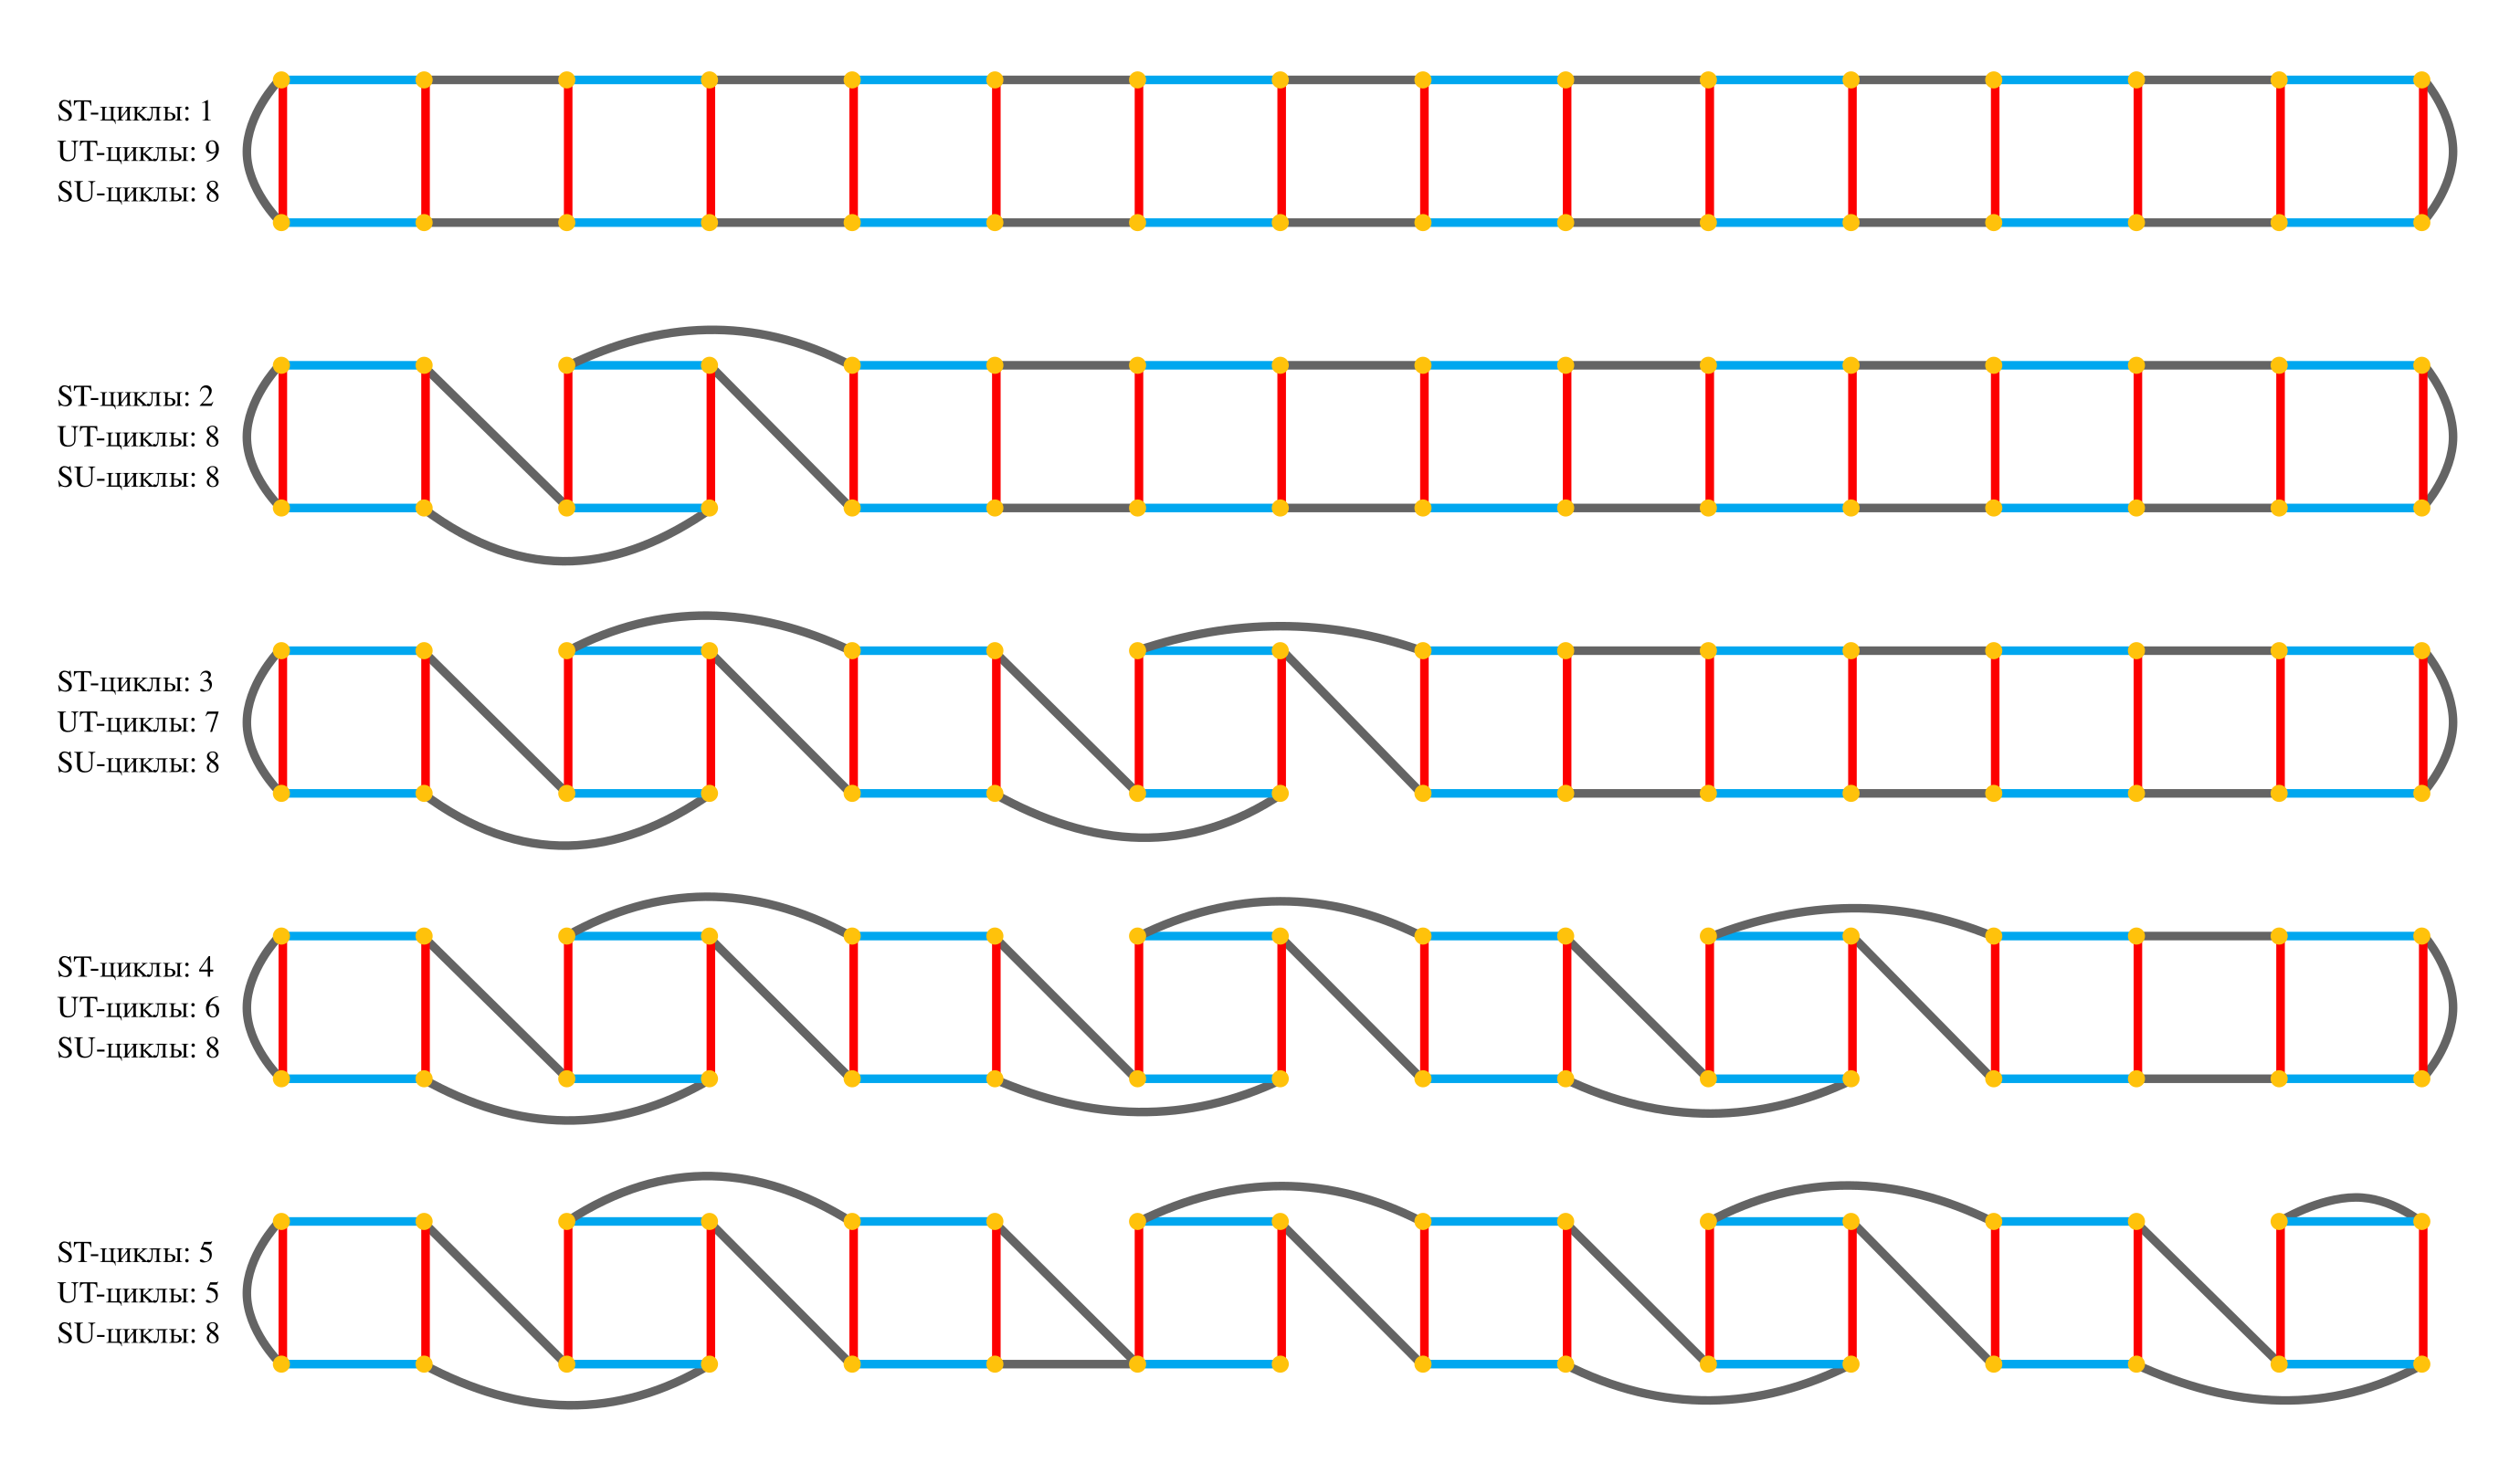
\includegraphics[width=\textwidth]{Spheres.png}
	\caption{Генератор графов для $e=2$ и $\sigma=8$ \label{overflow}}
	\end{figure}
	Ниже приведены примеры построения трёхцветных графов при $\sigma=8$ и $e=0$ и $e=-2$ для рис. (КАКОЙ НОМЕР) и для рис. (КАКОЙ НОМЕР) соответственно.
	\begin{figure}[ht!]
	\centering
	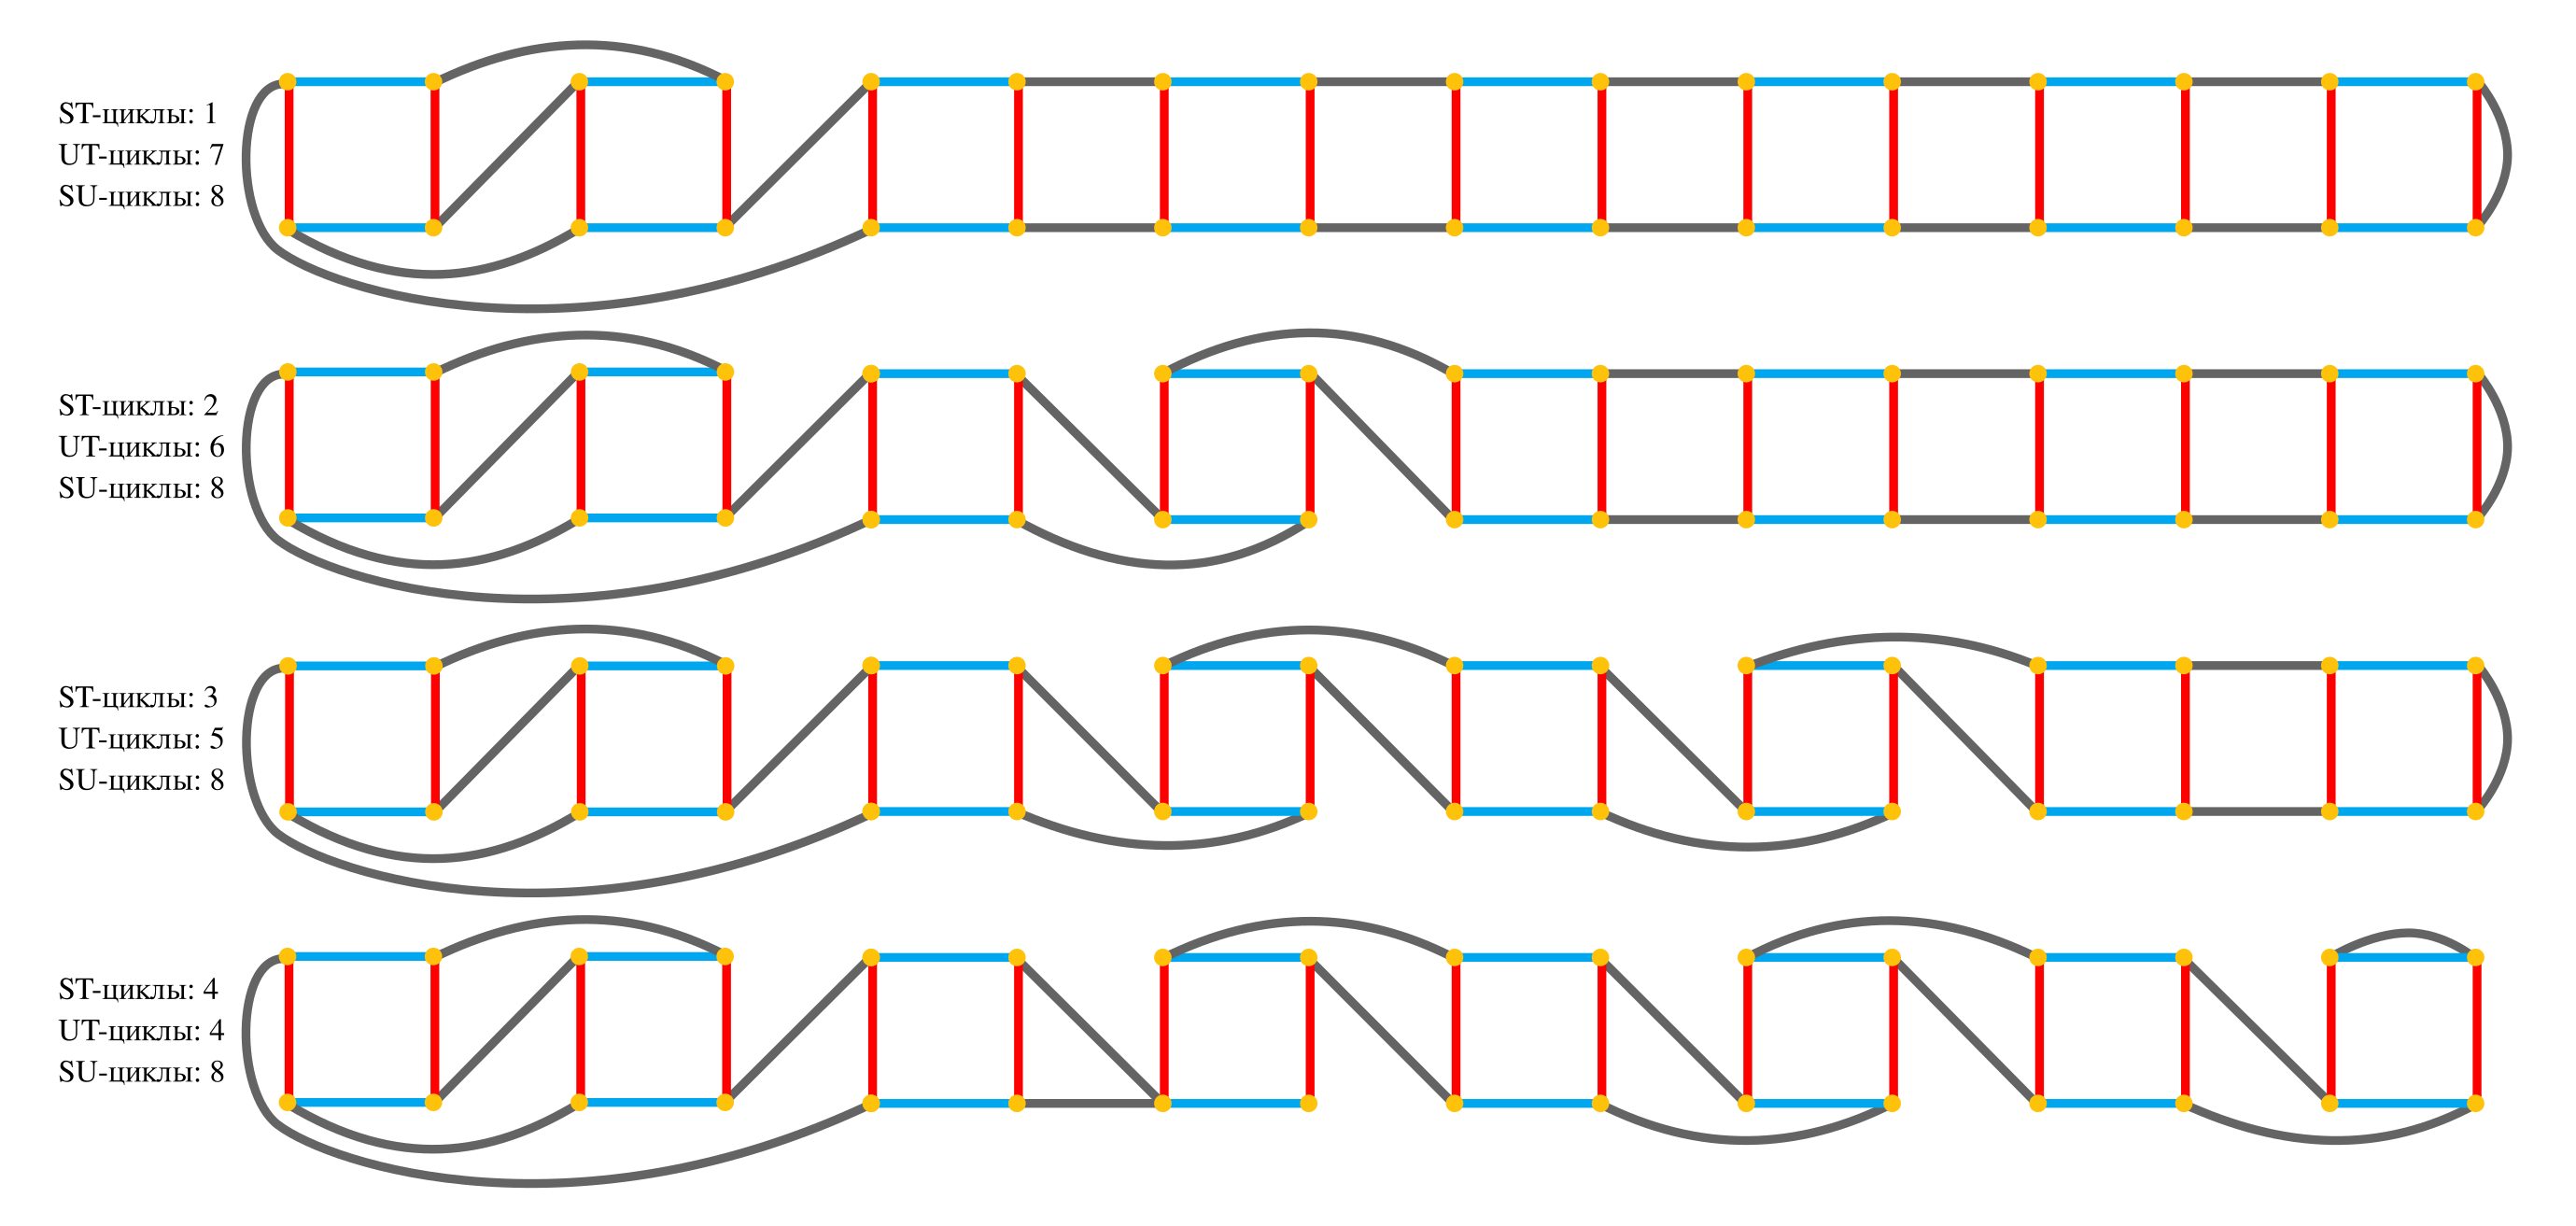
\includegraphics[width=\textwidth]{Torus.png}
	\caption{Генератор графов для $e=0$ и $\sigma=8$ \label{overflow}}
	\end{figure}
	\begin{figure}[ht!]
	\centering
	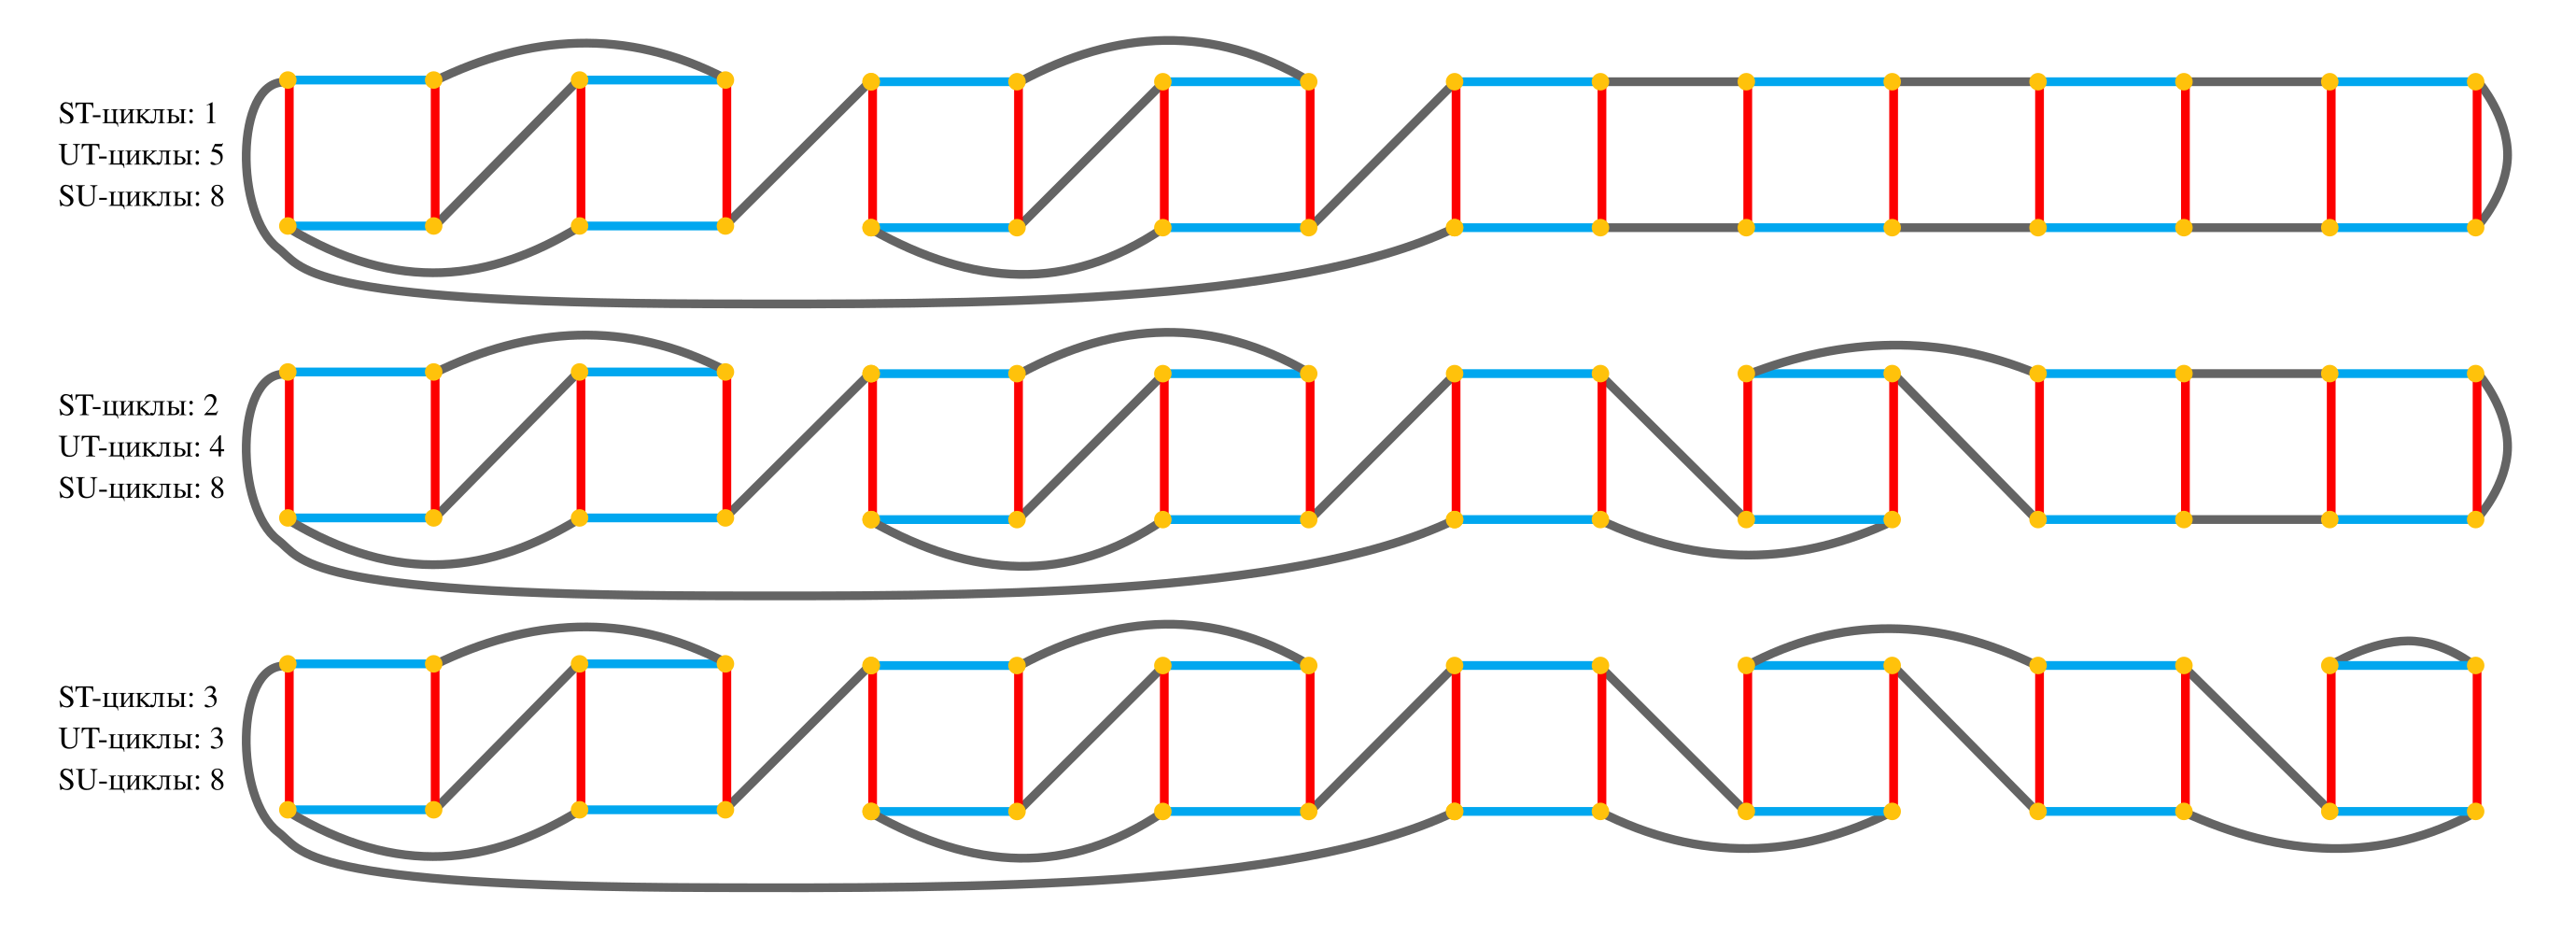
\includegraphics[width=\textwidth]{Double Torus.png}
	\caption{Генератор графов для $e=-2$ и $\sigma=8$ \label{overflow}}
	\end{figure}
	\subsection{Поиск соседних неподвижных точек}
	Нам дан корректный трёхцветный граф, для дальнейшей визуализации динамической системы для каждой неподвижной точки необходимо найти соседние, то есть соединённые с данной неподвижной точкой сепаратрисой, неподвижные точки. Для этого реализуем функцию $find \textunderscore neighbors$, которая принимает на вход корректный трёхцветный граф, а выдаёт вектор, состящий из стоков, сёдел и источников, а также их соседей в правильной последовательности.
	Для начала найдём все ST-, UT-, SU-циклы в исходном графе. Напомним, что каждый ST-цикл соответствует источнику, UT-цикл - стоку, SU-цикл - седлу. Из построения трёхцветного графа следует, что циклы имеют общее красное или синее ребро тогда и только тогда, когда неподвижные точки, представляющие эти циклы, соединены сепаратрисой, причём порядок обхода сепаратрис вокруг неподвижной точки соответствует порядку обхода рёбер графа, а также что одно ребро лежит ровно в двух двухцветных циклах, поэтому, найдя все двухцветные циклы, будем идти по ним в порядке обхода и для красных и синих рёбер будем смотреть, в каком ещё двухцветном цикле они лежат, далее сопоставляем новому двухцветному циклу для ребра неподвижную точку, соответствующую этому циклу. Проделаем это для всех неподвижных точек, получим искомый вектор.
	\subsection{Нахождение сепаратрис}
	Представим сферу как прямоугольник -90, 90 x 0, 360 фи пси, где все точки из отрезка -90 х 0, 360 и из отрезка 90 x 0, 360 отождествлены между собой. Впоследствии при визуализации этот прямоугольник будем отображать на сферу по формуле (КАКОЙ?). Сепаратрисы будем представлять как пары, состоящие из цвета сепаратрисы, красная или синяя, и вектора координат, содержащего $a, a0, b, b0$ и при этом заданной формулой (КАКОЙ?). 
	
	\subsection{Unit-тестирование}
	\section{Графическая часть}
	\subsection{Работа с библиотекой Manim}
	Графическая часть программы, написанная в файле draw.py, отвечает за генерацию 3D-изображения дискретной динамической системы на сфере. $\\$
	В файле определён класс DynamicalSystemSphere, который в дальнейшем будет указываться при запуске графической части. $\\$
	Графическая часть работает по следующему алгоритму: $\\$
	1) Считывается информация о сепаратрисах, полученная в результате запуска алгоритмической части; $\\$
	2) Объявляется функция $func \textunderscore sphere$, задающая параметрически поверхность сферы: $\\$
		x = r * cos(u) * sin(v) - x0 $\\$
		y = r * sin(u) * sin(v) - y0 $\\$
		z = r * cos(v) - z0 $\\$
	3) Объявляется функция $construct$, которая отвечает непосредственно за генерацию 3D-изображения. При помощи библиотеки Manim создаются поверхность сферы и оси OX, OY и OZ. Далее каждая сепаратриса, разбитая на 3 равные части, отличающиеся по цвету: более яркий красный и синий цвет соответствуют близости к стокам и источникам соответственно, а бледные оттенки этих цветов соответствуют близости к седлу, по отдельности добавляется на поверхность сферы следующим образом: $\\$
		сепаратриса, заданная параметрически на прямоугольнике значениями $a, a0, b, b0$, отображается на поверхность сферы по правилу: $\\$
			x = cos(pi * (t * b + b0) / 180) * sin(pi * (t * a + a0) / 180) $\\$
			y = cos(pi * (t * b + b0) / 180) * cos(pi * (t * a + a0) / 180) $\\$
			z = sin(pi * (t * b + b0) / 180) $\\$
		где t принадлежит [0, 1]. $\\$
	Для получения 3D-изображения объявляется полный оборот камеры вокруг сферы.
	\subsection{Запуск и результат работы программы}
	Для запуска генерации 3D-изображения необходимо: $\\$
	1) При помощи терминала установить библиотеку Manim на компьютер, если эта библиотека ещё не установлена. $\\$
	2) Предварительно запустить алгоритмическую часть с введённым в неё корректным трёхцветным графом. $\\$
	3) При помощи терминала перейти в каталог с файлом draw.py. $\\$
	4) Запустить графическую часть при помощи команды: $\\$
		manim -pqh draw.py DynamicalSystemSphere - для генерации изображения высокого качества; $\\$
		manim -pql draw.py DynamicalSystemSphere - для генерации изображения низкого качества.
	\section{Ссылка на репозиторий в Github}
	Ссылка: $https://github.com/dan1lka257/graphs \textunderscore and \textunderscore algorithms/tree/main$
	\section{Список литературы}
	1) Гринес В.З., Капкаева С.Х., Починка О.В. Трёхцветный граф как полный топологический инвариант для градиентно-подобных диффеоморфизмов поверхностей - Математический сборник, 2014, том 205, номер 10, 19-46 с.
	2) К.Патон. Алгоритм нахождения базы циклов для неориентированного графа - Communications of the ACM 12, 1969 - 514-518 с.
\end{document}